\documentclass{article}
\usepackage[table]{xcolor}
\usepackage{subfig}
\usepackage{framed}
\usepackage{tikz}
\usepackage{graphicx}
\usepackage{minted}
\usepackage{hyperref}
\usepackage{float}
\usepackage{algorithm}
\usepackage{algpseudocode}

\hypersetup{
    colorlinks,
    citecolor=black,
    filecolor=black,
    linkcolor=black,
    urlcolor=black
}

\title{\Huge \textbf{Projet Mansuba}}
\author{Louis Peyrondet, Samuel Khalifa}
\date{}

\usetikzlibrary{graphs}
\begin{document}
    \maketitle

    \vspace{3cm}

{\centering \LARGE
EI5PR103 - Projet d'algorithmique et de programmation n°1\par
Responsable : David Renault \par
Département Informatique \par
S5 - Année 2022/2023 \par
}

\begin{figure}[btp]
\centering 
\includegraphics[width=8cm]{images/logo_em.jpg}
\end{figure}

\newpage
\tableofcontents

    \section*{Presentation}

Le projet de cette année, Mansuba, était la réalisation d'un \emph{framework} pour la création de jeux de plateau.
Le développement du projet s'est déroulé entre le 8 novembre 2022 et le 13 janvier 2023. 

Notre projet contient plusieurs fonctionnalités comme : Plusieurs type de pièce de jeu, le changement des relations en cours de jeu, 
un système de capture et d'évasion, une interface en ligne de commande pour l'interaction, le calcul des meilleurs coups jouable ainsi que 
des configurations prédéfinies.


    \section{Choix techniques}
Durant ce projet, nous avons copieusement abusé des mallocs. Cela pose
certains soucis de gestion de la mémoire (principalement des \emph{memory leaks})
détectables avec \verb|valgrind|, mais cela nous avantage grandement.
En effet, cela nous permet de faire des
objets "persistents". Ils restent en mémoire jusqu'à la fin du programme
ou libération de la mémoire. Cela nous donne l'option d'utiliser des
structures de données génériques. Une structure de données

\subsection{Modularité}
Nous avons séparé notre projet en plusieurs modules, ce qui nous permet d'avoir une meilleure organisation au niveau des fichiers
ainsi que dans la logique des composants. Nos structures de données ne sont utilisables qu'à l'aide d'interfaces ce qui permet de changer
l'implémention sans perturber les autres modules. 


\subsection{Structure du jeu}

\begin{minted}{c}
typedef struct {
    uint turn;
    uint max_turns;
    player_t *current_player;
    enum victory_type victory_type;
    struct world_t *world;
    array_list_t *captured_pieces_list;
    array_list_t *starting_position;
} game_t;
\end{minted}


Notre structure game\_t comprend tous les éléments nécessaires pour le déroulement
d'une partie du jeu.
Avec le recul et l'avancement dans le projet une amélioration que nous voulions mettre en place mais n'avons
pas eu le temps était de remplacer les champs captured\_pieces\_list et starting\_pos par des tableaux d'array\_list.
Les tableaux seraient de taille nombre\_de\_couleurs afin d'avoir une array\_list pour chaque couleur ce qui permet
une séparation entre les pièces capturées selon leurs couleurs. Le bénéfice d'un tel changement est 
d'éviter les parcours inutiles, par exemple, lors de la libération de pièces, nous devons dans un premier temps
parcourir la liste des pièces capturées afin de récupérer seulement celles de la couleur du joueur alors
qu'avec la nouvelle implémentation cette étape n'est pas nécessaire donc il y aurait un gain de temps et
une simplification du code.  


\subsection{Implémentation des structures de données}
Premièrement toutes nos structures de données (sauf l'arbre par manque de temps)
n'exportent pas l'implémentation de la structure sous-jacente. Dans le \verb|.h|, il n'y a que la déclaration
du nom de la structure, pas son implémentation. Cela nous permet de réaliser un couplage faible
entre les différents fichiers utilisant ces structures de données.
\subsubsection{Tableau dynamique}
Pour le tableau dynamique, nous avons besoin des opérations standards 
sur une liste, à savoir l'ajout, la suppression, l'insertion, l'affectation, et la récupération.
Vu que c'est un tableau sous-jacent, l'insertion et la suppression seront en complexité en temps O(n).
Il faut déplacer tous les éléments dans le tableau.
Ensuite, la récupération et affectation seront en complexité en temps O(1).
Enfin, l'ajout d'un élément à la fin du tableau sera en temps moyen O(log(n)).
En effet, lorsqu'on dépasse la taille du tableau, on doit allouer un nouveau tableau
pouvant contenir tous les éléments précédents et l'élément à ajouter.
L'approche naïve serait d'allouer un nouveau tableau de taille n+1. Le problème,
c'est que si on veut rajouter pas 1, mais 2 élements, on devra allouer 2 nouveaux tableaux, et donc recopier la liste complète 2 fois.
L'approche un peu plus subtile (celle qu'on a choisie), c'est de doubler la taille du tableau.
Cela évitera de devoir copier tous les éléments de la liste trop souvent. Au désavantage de gâcher un peu plus de mémoire.
\subsubsection{Arbre}
Pour notre arbre, nous avons choisi de l'implémenter avec une structure récursive.
Un noeud possède une valeur, une liste d'enfants et un parent.
Nous avons opté pour un double chaînage car nous en avions besoin pour remonter l'arbre
lors du calcul des mouvements possibles\textsuperscript{\ref{fig:example-moves}}.
Pour la liste des enfants, nous avons utilisé le tableau dynamique défini précédemment.
\subsubsection{Liste chaînée}
Nous avions aussi besoin d'une liste chaînée.
En effet, contrairement au tableau dynamique, l'affectation et la récupération sont en complexité O(n).
Mais, les opérations d'insertion et de suppression sont en O(1). En gardant
des pointeurs vers le dernier et premier élément de la liste, cela nous permet d'avoir un type
qui peut fonctionner comme une pile et une file en temps constant. Nous avions
particulèrement besoin d'une file pour le parcours en largeur\textsuperscript{\ref{alg:BFS}}.
\subsection{Structure des fichiers}

    \section{Principaux algorithmes}
\subsection{Mouvements des pièces}
Pour le mouvement des pièces, nous avons choisi de le représenter comme
un arbre des positions. Un noeud et ses parents représentent tout le 
chemin pour arriver à la position au noeud. Voici un exemple :

\begin{figure}[H]
    \centering
    \begin{tabular}{|c|}
        \hline
        idx \\
        \hline
    \end{tabular} : case libre
    \begin{tabular}{|c|}
        \hline
        \cellcolor{gray}\color{white}idx \\
        \hline
    \end{tabular} : pion
    \begin{tabular}{|c|}
        \hline
        \cellcolor{green}\color{black}idx \\
        \hline
    \end{tabular} : pion à jouer
    \\
    \subfloat[Grille de jeu]{
        \begin{tabular}{|c|c|c|c|c|}
            \hline
            0                               & \cellcolor{gray}\color{white}1 & 2                              \\\hline
            \cellcolor{gray}\color{white}3  & 4                              & \cellcolor{gray}\color{white}5 \\\hline
            \cellcolor{green}\color{black}6 & \cellcolor{gray}\color{white}7 & 8                              \\\hline
        \end{tabular}
    }
    \\
    \raisebox{-0.5\height}{
        \subfloat[Arbre des mouvements possibles]{
            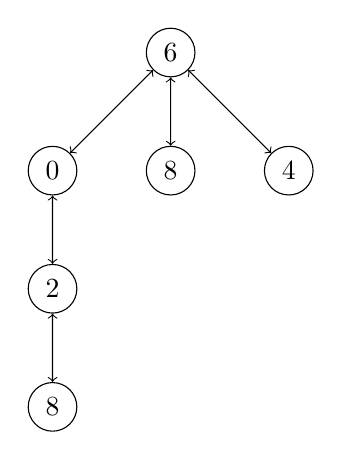
\begin{tikzpicture}[nodes={draw, circle}]
                \node {6}
                child {
                        node {0} edge from parent [<->]
                        child {
                                node {2} edge from parent [<->]
                                child {
                                        node {8} edge from parent [<->]
                                    };
                            };
                    }
                child {node {8} edge from parent [<->]}
                child {node {4} edge from parent [<->]};
            \end{tikzpicture}
        }
    }
    \hspace{1.5em}
    \raisebox{-0.5\height}{
        \subfloat[Ensemble des mouvements possibles]{
            \begin{tabular}{ ccccccccc }
                0 & 1 & 2 & 3 & 4 & 5 & 6 & 7 & 8 \\\hline
                \multicolumn{1}{|c|}{1}
                & \multicolumn{1}{|c|}{0} 
                & \multicolumn{1}{|c|}{1} 
                & \multicolumn{1}{|c|}{0} 
                & \multicolumn{1}{|c|}{1} 
                & \multicolumn{1}{|c|}{0} 
                & \multicolumn{1}{|c|}{0} 
                & \multicolumn{1}{|c|}{0} 
                & \multicolumn{1}{|c|}{1} 
                \\\hline
            \end{tabular}
        }
    }
    \caption{}
\end{figure}

Cet exemple nous montre 2 représentations des déplacements possibles pour
le pion à l'indice 6 sans compter les captures. L'ensemble à quelques avantages comparé à l'arbre.
Premièrement, pas besoin d'allocation dynamique, on peut juste faire un ensemble statiquement alloué
qui a la taille du monde. Ensuite, on a une complexité O(1) pour voir si on n'est pas déjà allé sur une case
lors de sauts multiples. L'implémentation en arbre, elle, doit être allouée dynamiquement,
et il y a une complexité O(h) pour voir si nous ne sommes pas déjà allé sur une case (grâce au double chaînage).
Mais, contrairement à l'implémentation avec un ensemble, nous pouvons savoir
exactement quel chemin a été emprunté pour aller à une position. Prenons les sauts
multiples pour arriver à la case 8. Dans le jeu des dames chinoises classique,
il y aurait une stratégie : est-ce que je prends le pion à la case 7, ou ceux aux cases 1 et 5 ?
Or, l'implémentation en ensemble ne permet pas de définir quel chemin nous avons emprunté.
Tandis qu'avec l'implémentation en arbre, il suffit de remonter l'arbre pour voir quel chemin nous avons emprunté.
Même si l'arbre complexifie le problème, il permet de rendre les mouvements bien plus génériques.


\subsection{Choix des meilleurs mouvements}
\subsubsection{BFS}
Pour pouvoir calculer les meilleurs mouvements, nous avons utilisé un Parcours en Largeur (Breadth First Search : BFS) sur le plateau. 
Premièrement on initialise la distance de toutes les cases avec une valeur maximale puis
le principe est de créer une file dans laquelle on ajoute toutes les positions de départ d'une couleur.
Ensuite tant que la file n'est pas vide, on récupère la position en tête, et pour chacun de ses voisins, 
si sa distance est inférieure on met à jour sa distance, qui est maintenant égale à la distance de notre position+1,
puis on l'enfile.
Ainsi chaque case se voit attribuer sa distance à la position de départ la plus proche pour une couleur. 
 
Cela nous permet d'avoir la distance d'une case donnée vers la position de départ d'une couleur avec une certaine relation. 
Ensuite il suffit de changer la relation et de relancer l'algorithme.

\begin{algorithm}
    \caption{BFS pour calculer les distances}\label{alg:cap}
    \begin{algorithmic}
    \Require $C \in couleurs$
    \Require $R \in relations$
    \Require $positions\_de\_depart\_de\_C \in file $
    \Require $Toutes\ les\ distances\ des\ autres\ positions\ initialisees\ au\ max$
    \While{$ !estVide(file) $}
    \State $position \gets tete(file)$
    \State $voisins \gets get\_neighbors(position)$
    \For{\texttt{voisin in voisins}}

    \If{$distance(position) + 1 < distance(voisin)$ }
        \State $set\_distance(distance(position) + 1, voisin, C, R)$
        \State $file \gets ajout(file, voisin)$
    \EndIf
    \EndFor
    \State $file \gets defiler(file)$
    \EndWhile
    \end{algorithmic}
\end{algorithm}

\subsubsection{Table de correspondance}

Ces distances sont enregistrées dans un tableau ce qui nous permet d'avoir une table de correspondance (\emph{lookup table}),
pour avoir en temps constant toutes les distances lors d'une partie vu que celle-ci est calculée lors de l'initialisation
du programme. Concernant la complexité en espace, elle réserve 
taille\_du\_monde * nombre\_de\_couleurs * nombre\_de\_relations * taille\_short\_int octets. Pour un jeu standard de configuration
 HEIGHT=4 WIDTH=5, avec 2 joueurs et 3 relations différentes, la taille allouée est de 240 octets, ce qui est correct.
Nous avons choisi d'utiliser des short int (2 octets) à la place des int (4 octets) pour réduire la taille totale allouée,
le seul inconvéniant que cela ajoute est que la distance maximale pouvant être enregistrée sans overflow est de \emph{65 535} mais cela
est largement suffisant pour nos utilisations.

Pour choisir le meilleur coup à jouer, on regarde parmi toutes les positions atteignables depuis 
notre case et on choisit celle dont la distance est la plus petite dans notre table de correspondance.

Nous avons opté pour une représentation de cette table par un tableau contigu en mémoire afin de favoriser le cache cpu
lors du BFS avec la localité spatiale et temporelle des accès mémoire. 

\begin{figure}[H]
\centering
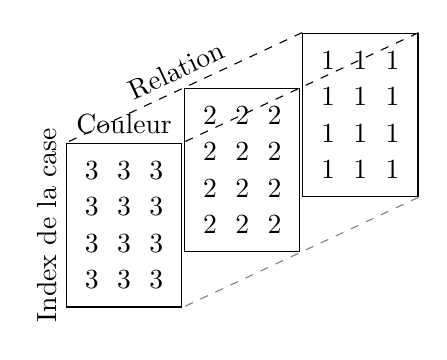
\begin{tikzpicture}
    \def\xs{1.5} %shift in x direction
    \def\ys{0.7} %shift in y direction
    \def\nm{3} % number of 2d matrices in the 3d matrix
    \foreach \x in {1,2,...,\nm}
    {
    
    \matrix [draw, % for the rectangle border
             fill=white, % so that it is not transparent
             ampersand replacement=\&] %see explanation
    (mm\x)%give the matrix a name
    at(-\x * \xs, -\x * \ys) %shift the matrix
    {
        \node {\x}; \& \node {\x}; \& \node {\x};\\
        \node {\x}; \& \node {\x}; \& \node {\x};\\
        \node {\x}; \& \node {\x}; \& \node {\x};\\
        \node {\x}; \& \node {\x}; \& \node {\x};\\
    };
    }
    
    \draw [dashed,black](mm1.north west) -- node[sloped,above] {Relation} (mm\nm.north west);
    \draw [dashed,black](mm1.north east) -- (mm\nm.north east);
    \draw [dashed,gray](mm1.south east) -- (mm\nm.south east);

    \node [rotate=90][above] at (mm3.west) {Index de la case};
    \node [above] at (mm3.north) {Couleur};
    
\end{tikzpicture}
\caption{Représentation de la table de correspondance}
\end{figure}



    \section{Tests}

Tout les tests du projet sont rassemblés dans le dossier tst/ . 

\subsection{Structures de données}
Pour chacune des structures de données que nous avons utilisées (arbres, array\_list, liste chaînée),
il existe un fichier de test correspondant. Cela nous permet de nous assurer que ces structures, qui
forment la base de notre projet, fonctionnent sans problèmes. Dans ces tests on s'assure que les fonctions
donnent le résultat attendu dans les cas classiques ainsi que dans des cas limites tel que la suppression 
dans une liste vide. 

Ces tests sont également examiné par \emph{valgrind} afin d'être sûr qu'il n'y a pas 
de fuite de mémoire.

\subsection{Modules principaux}
Pour pouvoir tester nos modules principaux, on met en place une situation spécifique puis on appelle une des 
fonctions du module et on compare cette nouvelle situation après l'éxécution à celle qui est attendu.

Certains module n'ont cependant pas de test car difficilement réalisable. C'est le cas par exemple de notre
module player\_handler, qui s'occupe de gérer l'interaction d'un joueur à travers le terminal, vu que simuler
les entrées n'est pas trival et surtout que c'est un module de haut niveau donc presque aucun module n'en dépend.


    \section{Mots de fin}
Pour finir ce rapport, nous aimerions parler de ce que nous avons appris, ce qui nous a plu dans ce projet, et ce qui nous a déplu.
\subsection{Ce que nous avons appris}
Nous n'avons pas tant appris sur le plan technique comparé à nos camarades,
cependant, cela peut s'expliquer par notre parcours. En effet, l'un a fait une licence informatique, tandis que l'autre a fait un DUT Informatique.
Nous avions donc déjà un fort bagage technique. Néanmoins, ce projet nous a tout de même permis de consolider nos connaissances,
et même d'apprendre de toutes nouvelles choses. Par exemple, nous avons appris que pour déclarer une fonction sans paramètres,
il fallait la déclarer comme ceci : \verb|type nom(void);|. En effet, si
nous ne mettons pas le \verb|void|, cela n'est plus un prototype de fonction.
Cela peut donc causer plusieurs soucis au niveau de la compilation (incohérences \verb|.h| et \verb|.c|).
Pour détecter ce type d'erreurs, nous avons donc appris qu'il fallait utiliser le tag gcc \verb|-Wstrict-prototypes|.
De plus, nous nous sommes efforcés d'utiliser des principes de programmation en C plutôt obscurs,
tels que ne pas utiliser d'assert dans le code en production, car avec un tag gcc, on peut désactiver les assert.
Nous avons donc défini une macro qui permet de vérifier si un malloc a bien alloué de la mémoire, sinon, le programme plante.

\subsection{Les + du projet}
On était relativement libre sur le projet. On pouvait implémenter une solution algorithmique différente de celle proposée,
et nous avions un minimum à implémenter, mais pas un maximum. De plus, la seule structure de code vraiment imposée est
celle de départ (même si cela nous a bien embêté). Aussi, nous étions bien encadrés,
dès que nous avions une question, l'enseignant nous répondait de façon approfondie et compréhensible.
De plus, les solutions algorithmiques proposées étaient intéressantes, voire intriguantes.
Enfin, le sujet était intéressant dans son ensemble.

\subsection{Les - du projet}
Les fichiers \verb|.c| et \verb|.h| imposés étaient plutôt embêtants.
Nous en avons déjà parlé plus haut \textsuperscript{\ref{ssec:module-util}}, mais cela nous a forcé à faire un fichier 
\verb|util.h| alors que nous aurions pu mettre certains types dans 
\verb|neighbors.h| ou \verb|geometry.h|. Ensuite, le fait qu'il n'y ait pas 
d'\emph{Issue Board} sur la forge nous a forcé à créer un trello, ce n'est
pas si grave, mais tout de même embêtant.
    \section*{Annexe}

\end{document}